\section{Convolutional Neural Network}\label{sec:cnn}
In this section I will describe a Convolutional Neural Network architecture designed by me.

\subsection{Architecture}\label{sec:cnn-architecture}
The architecture is structured as follows:
\begin{itemize}
    \item \textbf{Input}: 256$\times$x256$\times$3
    \item \textbf{Convolution}: 32 filters of size 11$\times$11$\times$3 with stride 4 and padding valid
    \item \textbf{Max Pooling}: 2$\times$2 with no stride
    \item \textbf{Convolution}: 64 filters of size 5$\times$5$\times$96 with stride 1 and padding valid
    \item \textbf{Max Pooling}: 2$\times$2 with no stride
    \item \textbf{Flatten}
    \item \textbf{Dense}: 128 neurons
    \item \textbf{Dense}: 10 neurons
\end{itemize}

\subsection{Training}\label{sec:cnn-training}
I have trained two CNN models with different learning rates (0.001 and 0.0001) using the Adam optimizer.
It has been trained using Google Colab with a GPU runtime and the training took about 1 hour for each model.
The training and validation accuracy and loss are shown in Figure~\ref{fig:cnn-accuracy} and Figure~\ref{fig:cnn-loss}.

\begin{figure}[h]
    \centering
    \subfloat[\centering Learning Rate = 0.001]{{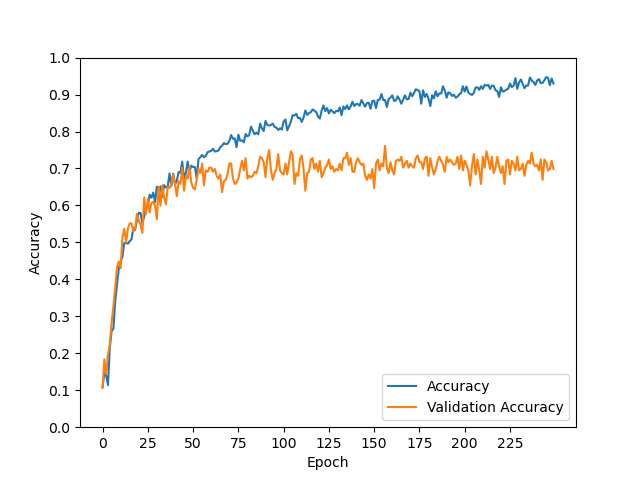
\includegraphics[width=0.45\textwidth]{../plot/lr-0001/cnn-accuracy.png}}}
    \qquad
    \subfloat[\centering Learning Rate = 0.0001]{{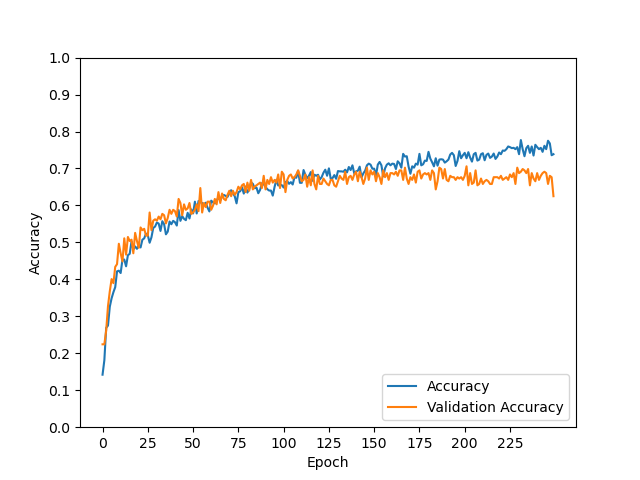
\includegraphics[width=0.45\textwidth]{../plot/lr-00001/cnn-accuracy.png}}}
    \caption{Training and validation accuracy for the CNN with different learning rates}\label{fig:cnn-accuracy}
\end{figure}

\begin{figure}[h]
    \centering
    \subfloat[\centering Learning Rate = 0.001]{{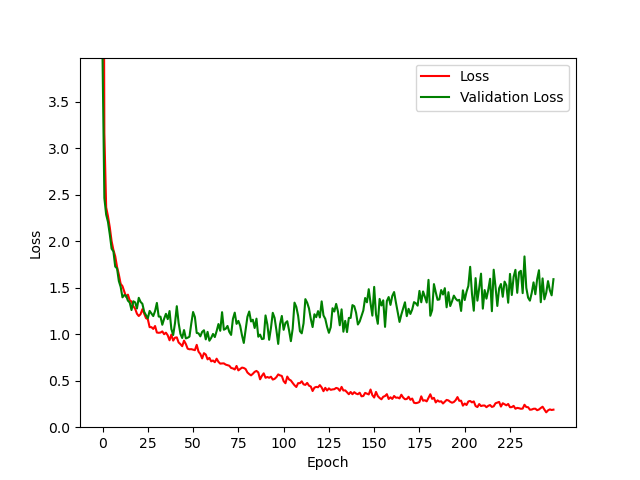
\includegraphics[width=0.45\textwidth]{../plot/lr-0001/cnn-loss.png}}}
    \qquad
    \subfloat[\centering Learning Rate = 0.0001]{{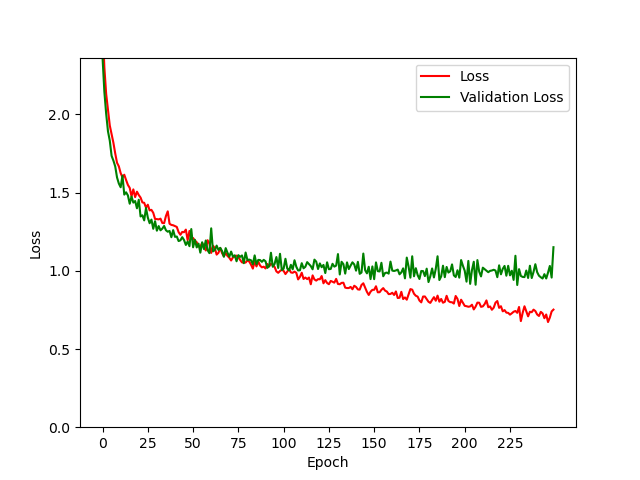
\includegraphics[width=0.45\textwidth]{../plot/lr-00001/cnn-loss.png}}}
    \caption{Training and validation loss for the CNN with different learning rates}\label{fig:cnn-loss}
\end{figure}

\subsection{Evaluation}\label{sec:cnn-evaluation}
The model was evaluated using the test dataset and the results are shown in the confusion matrix in Figure~\ref{fig:cnn-confusion-matrix}.
The accuracy, precision, recall, F1-score and AUC are shown in Table~\ref{tab:results-cnn}.

As we can see from the results, both the learning rates have similar results.
However, the model with a learning rate of 0.001 have a better accuracy and a better AUC.
In fact we can see from the confusion matrix that the model with a learning rate of 0.001 is able to classify better the classes.


\begin{table}[h]
    \centering
    \begin{tabular}{|c|c|c|c|c|c|}
        \hline
        \textbf{LR}     & \textbf{Accuracy} & \textbf{Precision} & \textbf{Recall} & \textbf{F1-Score} & \textbf{AUC} \\
        \hline
        \textbf{0.001}  & 0.6360            & 0.9825             & 0.9106          & 0.9451            & 0.8784       \\
        \hline
        \textbf{0.0001} & 0.6213            & 0.9305             & 0.9797          & 0.9545            & 0.6437       \\
        \hline
    \end{tabular}
    \caption{Evaluation of the CNN with different learning rates}\label{tab:results-cnn}
\end{table}

\begin{figure}[h]
    \centering
    \subfloat[\centering Learning Rate = 0.001]{{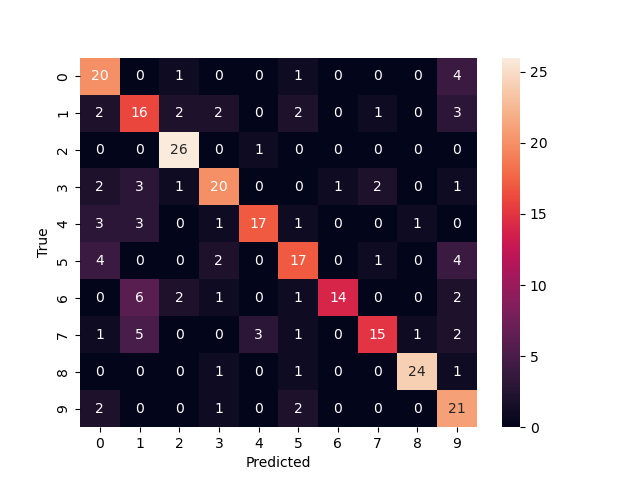
\includegraphics[width=0.45\textwidth]{../plot/lr-0001/cnn-confusion-matrix.png}}}
    \qquad
    \subfloat[\centering Learning Rate = 0.0001]{{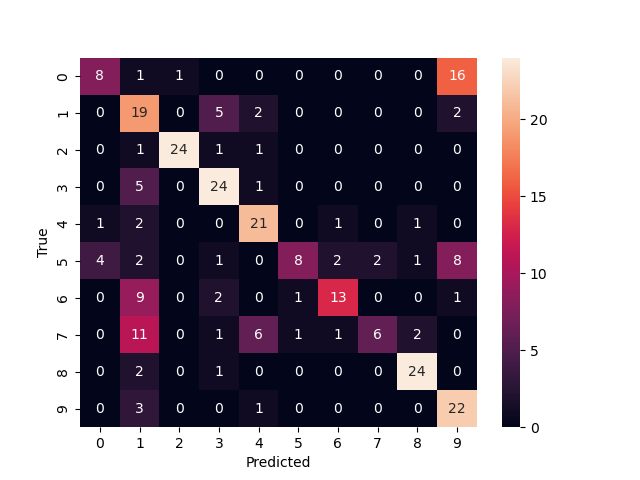
\includegraphics[width=0.45\textwidth]{../plot/lr-00001/cnn-confusion-matrix.png}}}
    \caption{Confusion matrix for the CNN with different learning rates}\label{fig:cnn-confusion-matrix}
\end{figure}